\documentclass[12pt,letterpaper]{article}

% Paquetes base
\usepackage[spanish]{babel}
\usepackage[utf8]{inputenc}
\usepackage[T1]{fontenc}
\usepackage{mathpazo}
\usepackage[margin=2.5cm]{geometry}
\usepackage{setspace}
\onehalfspacing
\usepackage{parskip}
\usepackage{microtype}
\usepackage{graphicx}
\usepackage{hyperref}
\hypersetup{colorlinks=true, linkcolor=black, urlcolor=blue, citecolor=black}

\usepackage{xcolor}
\usepackage{enumitem}
\usepackage{ragged2e}
\usepackage{float}
\usepackage{csquotes}
\usepackage{tabularx}
\usepackage{booktabs}
\usepackage{multirow}
\usepackage{amsmath}
\usepackage{amssymb}

% Encabezado/pie
\usepackage{fancyhdr}
\pagestyle{fancy}
\fancyhf{}

% Altura del encabezado para que quepa el logo (1.8 cm ~ 51pt)
\setlength{\headheight}{52pt}
% (Opcional) si ves el contenido muy abajo, puedes recuperar un poco de margen:
% \addtolength{\topmargin}{-8pt}

% Encabezado
\lhead{
\includegraphics[height=1.8cm]{Img/escudo.png}}
\chead{Universidad del Bío-Bío}
\rhead{\nouppercase{\leftmark}}

% Pie de página
\lfoot{Sistemas Digitales}
\cfoot{\thepage}
\rfoot{Grupo 8}

% Líneas superior e inferior
\renewcommand{\headrulewidth}{0.4pt}
\renewcommand{\footrulewidth}{0.4pt}

% Espaciado de títulos (aleja los títulos del encabezado)
\usepackage{titlesec}
\titlespacing*{\section}{0pt}{0cm}{-0.1cm}
\titlespacing*{\subsection}{0pt}{0.5cm}{-0.1cm}

% (Opcional) Sin numeración en títulos (y siguen en el índice)
\setcounter{secnumdepth}{0}

% (Opcional) Cambiar el nombre del índice a "Índice"
\addto\captionsspanish{\renewcommand{\contentsname}{Índice}}
\setlength{\footskip}{0.9cm}  % valor más chico → sube el pie



\begin{document}
	
	\begin{titlepage}
		\thispagestyle{empty}
		
		% ===== Bloque superior: escudo + institución =====
		\begin{center}
			\vspace*{-2cm} % margen superior discreto
			
\includegraphics[height=3.5cm]{Img/escudo.png}\\[-0.2cm]
			
			{\large Universidad del Bío-Bío}\\[-2pt]
			{\large Facultad de Ciencias Empresariales}\\[-2pt]
			{\large Ingeniería Civil en Informática}
		\end{center}
		
		\vspace{1cm}
		\vfill
		
		% ===== Bloque central: TÍTULO =====
		\begin{center}
			\rule{\textwidth}{0.5pt}\\[0.5cm]
			{\Huge \textbf{Informe de laboratorio N\textsuperscript{o}3}}\\[0.25cm]
			{\Large Circuito ADC y DAC }\\[0.1cm]
			\rule{0.65\textwidth}{0.5pt}
		\end{center}
		
		\vspace{2cm}
		
		% ===== Bloque inferior compacto: Asignatura, Profesor, Integrantes =====
    \begin{flushleft}
    \normalsize
    \begin{tabular}{@{}ll@{}}
                           & \\
    \textbf{Integrantes}   & : Oscar Illanes Garrido \\
                           & \hspace{0.12 cm} Gabriela Maureira Ocaña \\
                           & \hspace{0.12 cm}  Bastian Palma Navarrete \\
                           & \\
    \textbf{Docente}       & : Julio C. Alarcón Monteros \\
                           & \\
    \textbf{Asignatura}    & : Sistemas Digitales \\
                           & \\
    \textbf{Carrera}    & : Ingeniería Civil en Informática \\
    \end{tabular}
    \end{flushleft}
		
		\vfill
		\begin{center}
			\normalsize\textbf{Chillán, 4 de mayo de 2026.}
		\end{center}
	\end{titlepage}
	
    \newpage

    \tableofcontents
    
    \newpage

    \section{Introducción}

    En la actualidad, muchos sistemas electrónicos requieren trabajar tanto con señales analógicas como con señales digitales. Las señales analógicas están presentes de forma natural en el entorno y pueden representar magnitudes como sonido, temperatura, presión o voltaje, las cuales varían continuamente en el tiempo. Sin embargo, los dispositivos digitales requieren información en valores discretos para poder procesarla correctamente. Por esta razón, es necesario contar con métodos que permitan transformar una señal de un tipo a otro.

    Dentro de este proceso destacan los convertidores Analógico-Digital (ADC) y Digital-Analógico (DAC), componentes ampliamente utilizados en distintos equipos electrónicos. El ADC se encarga de convertir una señal analógica en un código binario, mientras que el DAC realiza la operación contraria, es decir, toma datos digitales y los transforma nuevamente en una señal analógica. En esta experiencia de laboratorio se trabajó con ambos dispositivos mediante la conversión de una señal triangular tipo diente de sierra y su posterior reconstrucción, utilizando el software Multisim para realizar la simulación.

    El presente informe se encuentra dividido en distintas secciones. En primer lugar, se presentan los objetivos de la actividad. Luego, se desarrolla el marco teórico necesario para comprender el funcionamiento de los convertidores utilizados. Posteriormente, se explica el diseño del sistema implementado y los cálculos previos esperados. Finalmente, se muestran y analizan los resultados obtenidos en la simulación, comparando la señal de entrada con la señal digitalizada y la señal reconstruida.
    
    \section{Objetivo general}
Comprender el proceso de conversión analógico-digital y digital-analógico mediante el diseño y simulación de un circuito ADC/DAC aplicado a una señal triangular diente sierra. 

    \section{Objetivos específicos}
    \begin{itemize}
        \item Determinar las características de digitalización de una señal analógica triangular diente sierra, analizando su resolución, frecuencia de muestreo y codificación binaria. 
        \item Diseñar y simular un circuito ADC/DAC en Multisim, verificando el correcto funcionamiento de cada etapa del sistema mediante indicadores LED y el osciloscopio.
        \item  Analizar la relación entre la señal analógica original, su representación digital y la señal analógica reconstruida por el DAC, estableciendo las diferencias y similitudes entre ellas. 
    \end{itemize}
    

    \newpage

    \section{Desarollo teórico}
    
    \subsection{Señales analogicas y Digitales }
    Para analizar el funcionamiento de un sistema de conversión ADC/DAC como el que se implemento en el presente laboratorio, es ideal comenzar por establecer las bases conceptuales que diferencian dos de las formas fundamentales de representar la información en electrónica: las magnitudes analógicas y las magnitudes digitales. 

    Según \cite{floyd2006fundamentos} , una magnitud analógica es aquella que puede adoptar cualquier valor dentro de un rango continuo, mientras que una magnitud digital es aquella que solo puede tomar un conjunto finito y discreto de valores. Esta distinción es el punto de partida de toda la electrónica digital moderna. La mayoría de los fenómenos físicos del mundo real —como la temperatura, la presión, la distancia, la velocidad del viento o la intensidad sonora— son de naturaleza analógica: varían de forma continua a lo largo del tiempo sin saltos bruscos entre un valor y otro. Si se midiera la temperatura de una habitación a lo largo del día, por ejemplo, se obtendría una curva suave y continua como la que se representa a continuación. 

    Las magnitudes físicas al ser continuas  plantea un desafió para los sistemas computacionales, que trabajan en un dominio estrictamente binario.  Este es precisamente el rol del transductor: un dispositivo que convierte una magnitud física (como presión, temperatura, luz o sonido) en una señal eléctrica analógica proporcional a ella. En el contexto del presente laboratorio, el equivalente a este transductor es el generador de señal que produce la onda triangular diente sierra de 0 a 16 V, representando una magnitud analógica que el sistema deberá procesar.

    A continuación se ilustra la diferencia fundamental entre una señal analógica continua y su representación discreta (muestreada):

    \begin{figure}[H] % El [H] en mayúscula obliga a la figura a quedarse AQUÍ
        \centering
        % Primera imagen (ocupa el 45% del ancho de la página)
        \begin{minipage}{0.5\textwidth}
            \centering
            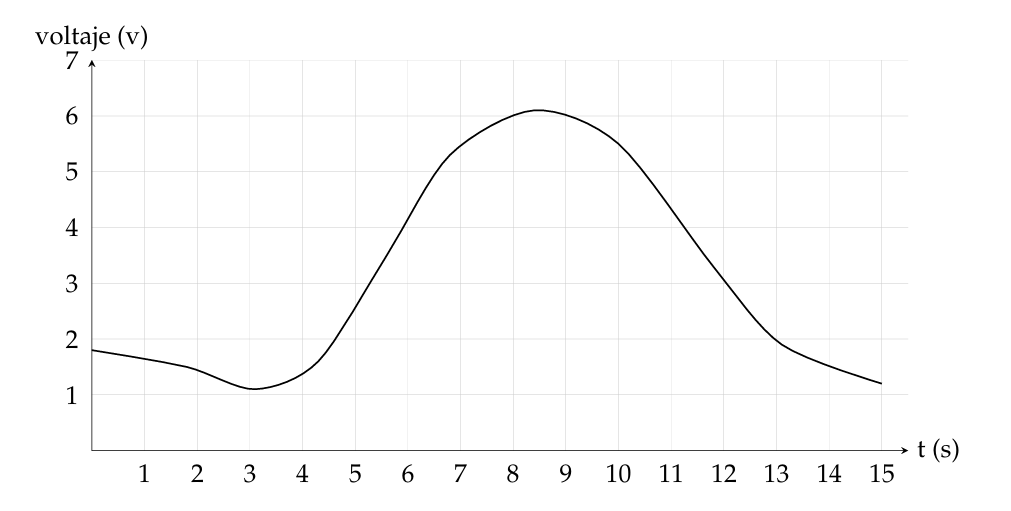
\includegraphics[width=\linewidth]{Img/1.png}
            \caption{Señal analogica continua}
            \label{fig:imagen_1}
        \end{minipage}\hfill % Este comando crea una separación automática y equitativa entre ambas imágenes
        % Segunda imagen (ocupa el otro 45%)
        \begin{minipage}{0.5\textwidth}
            \centering
            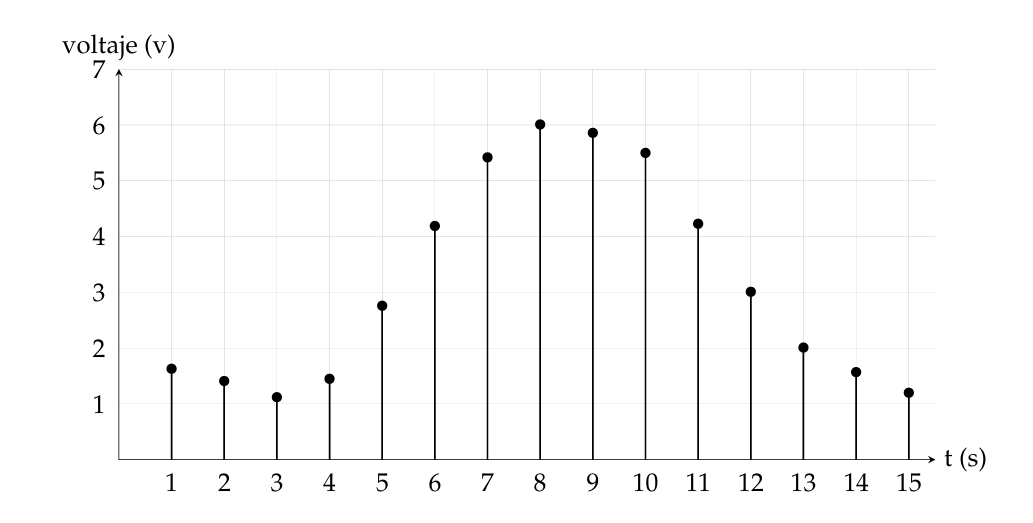
\includegraphics[width=\linewidth]{Img/2.png}
            \caption{Señal analógica muestreada}
            \label{fig:imagen_2}
        \end{minipage}
    \end{figure}
    
    \newpage


    Como se aprecia en la figura, la señal analógica (izquierda) es una curva suave y continua que puede tomar infinitos valores en cualquier instante del tiempo. La señal discreta (derecha) muestra solo los valores tomados en instantes específicos y equiespaciados, conservando la forma general de la señal original. Este proceso de tomar muestras en intervalos regulares es, precisamente, el primer paso hacia la digitalización. 

    Una vez captada la señal analógica mediante un transductor, el siguiente desafío es transformarla a un formato que los sistemas computacionales puedan procesar. Floyd (2006) señala que los circuitos electrónicos se dividen en dos grandes categorías: digitales, que trabajan con valores discretos, y analógicos, que emplean valores continuos.

    Las ventajas de trabajar en el dominio digital son significativas: los datos digitales pueden procesarse y transmitirse con mayor fiabilidad, su almacenamiento es más compacto y son mucho más inmunes al ruido eléctrico que las señales analógicas (Floyd, 2006). Un ejemplo que ilustra la integración de ambos dominios es el reproductor de CD, donde la música digital almacenada en el disco es convertida por un DAC en una señal analógica audible, mientras que el proceso de grabación utilizó originalmente un ADC para el camino inverso.

    En síntesis, los convertidores ADC y DAC son el puente tecnológico que permite que el mundo físico continuo y los sistemas digitales discretos coexistan en aplicaciones reales.

    \subsection{El proceso de muestreo}
    Para que la representación discreta sea fiel a la señal original, la frecuencia con que se toman las muestras debe ser suficientemente alta. Este criterio esta definido por el Teorema de Nysquit-Shannon, que establece que la frecuencia maxima presente en la señal analogica (fmax).
    
    \begin{equation}
        f_s \ge 2 \cdot f_{max}
        \label{Eq:fs}
    \end{equation}

    Donde:

    \begin{itemize}
        \item $f_s$: Frecuencia de muestreo (número de muestras por segundo)
        \item $f_{max}$: Frecuencia máxima presente en la señal analógica 
    \end{itemize}
    
    Si esta condición no se cumple, ocurre un fenómeno llamado aliasing, en el que la señal reconstruida presenta distorsiones que la hacen irreconocible respecto a la original. En cambio, cuando se respeta el teorema, la señal puede reconstruirse con total fidelidad a partir de las muestras.

    En el contexto de este laboratorio, la señal de entrada es una onda triangular diente sierra de 50 Hz. Aplicando el teorema, la frecuencia de muestreo mínima teórica sería de 100 Hz. Sin embargo, el sistema utiliza una frecuencia de muestreo de 1000 Hz mediante una señal cuadrada aplicada al pin SOC del ADC, lo que equivale a 20 muestras por ciclo de la señal. Esta relación garantiza una representación precisa y ampliamente superior al mínimo requerido.

    \subsection{Cuantificacion y resolucion }
    Una vez obtenidas las muestras de la señal analógica, el siguiente paso es asignarles un valor numérico que pueda representarse en formato binario. Este proceso se denomina cuantificación y consiste en mapear cada valor de voltaje muestreado a uno de los niveles discretos disponibles en el convertidor.

    La cantidad de niveles disponibles depende directamente del número de bits del convertidor. Para un ADC de n bits, el número total de niveles es $2^n$. El voltaje mínimo que puede distinguir el sistema entre un nivel y el siguiente se denomina voltaje de resolución o tamaño del escalón, y se calcula como:
    
    \begin{equation}
        V_{res} = \frac{V_{ref+} - V_{ref-}}{2^n}
        \label{Eq:Vres}
    \end{equation}

    Donde:
    
    \begin{itemize}
        \item $V_{ref+}$: Voltaje de referencia positivo
        \item $V_{ref-}$: Voltaje de referencia negativo
        \item $n$: Número de bits del ADC
    \end{itemize}
    
    A menor voltaje de resolución, más pequeños son los escalones y más fiel es la representación de la señal original. Sin embargo, dado que los valores analógicos son continuos y los niveles digitales son discretos, siempre existirá una pequeña diferencia entre el valor real de la señal y el valor digital asignado. Esta diferencia se conoce como error de cuantización, cuyo valor máximo teórico es de ±½ Vres, equivalente a la mitad de un escalón.

    A mayor número de bits, menor es el voltaje de resolución y menor el error de cuantización, lo que se traduce en una representación más fiel de la señal original. Este es el motivo por el que los sistemas de alta precisión emplean convertidores de 12, 16 o más bits.

    Sin ninguna mención a valores del laboratorio, queda puramente teórico. Avísame si quieres que revise las demás secciones bajo ese mismo criterio.

    \subsection{El Convertidor analogico-digital(ADC)}
    El convertidor analogico-digital(ADC) es el componente encargado de transformar una señal de voltaje continua en su equivalente representación binaria, integrando en un único dispositivo los procesos de muestreo y cuantificación descritos anteriormente.

    Sus terminales fundamentales son: la entrada de voltaje inicial, que recibe la señal analógica a convertir; las entradas $V_{ref+}$ y $V_{ref-}$, que definen el rango de voltaje dentro del cual opera el convertidor, saturando al código máximo o mínimo cualquier valor que quede fuera de ese rango; el pin SOC (\textit{Start of Conversion}), que recibe una señal de reloj externa que determina el ritmo al que se realizan las conversiones; y las salidas $D_0$ a $D_7$, que entregan el código binario resultante de cada conversión.
 
    \subsection{El convertidor digital-Analogico(DAC)}
    El convertidor digital-analógico (DAC) realiza el proceso inverso al ADC: toma un código binario y lo transforma en un voltaje analógico proporcional. Es fundamental en cualquier sistema que deba entregar una salida continua al mundo físico a partir de datos digitales, como altavoces, actuadores o pantallas.

    Su principio de funcionamiento consiste en ponderar cada bit del código de entrada según su peso posicional en el sistema binario y sumarlos para producir un voltaje de salida. El bit más significativo  aporta la mayor contribución, mientras que el bit menos significativo, aporta la menor. La señal resultante no es perfectamente continua, sino que presenta una forma escalonada característica del proceso de cuantización, donde cada nivel se mantiene constante hasta que llega el siguiente código.

    \subsection{Señal Triangular diente Sierra}
    La señal triangular diente sierra es una forma de onda periódica caracterizada por una rampa lineal ascendente seguida de una caída abrupta e instantánea de vuelta al valor inicial. A diferencia de una onda sinusoidal, que varía de forma suave y simétrica, la diente sierra sube linealmente y cae de manera abrupta, lo que le da su nombre al asemejarse al perfil de los dientes de una sierra.

    Esta señal resulta especialmente útil en el estudio de convertidores ADC, ya que su rampa lineal permite observar cómo el código binario de salida aumenta de forma progresiva y ordenada a medida que el voltaje de entrada crece, facilitando la verificación del comportamiento del sistema.
 
    \subsection{Relacion entre entrada y codificacion de salida}
    La relación entre el voltaje analógico de entrada y el código digital que entrega el ADC es directa y proporcional. Para un ADC de n bits con voltaje de referencia mínimo Vmin y voltaje de resolución Vres, el valor decimal equivalente al código de salida se calcula como: 
    
    \begin{equation}
        D_{10} = \frac{V_{in} - V_{min}}{V_{res}}
        \label{Eq:D10}
    \end{equation}

    donde:
    \begin{itemize}
        \item $D_{10}$: Valor decimal del código de salida
        \item $V_{in}$: Voltaje de entrada
        \item $V_{min}$: Voltaje mínimo de referencia
        \item $V_{res}$: Voltaje de resolución
    \end{itemize}
    
    El proceso inverso también es válido: dado un código binario de salida, es posible estimar el voltaje analógico que lo generó despejando la misma ecuación:
    
    \begin{equation}
        V_{in} = (D_{10} \cdot V_{res}) + V_{min}
        \label{Vin}
    \end{equation}
    
    Cabe destacar que el ADC no realiza redondeo sino truncamiento, por lo que el valor decimal obtenido se aproxima siempre hacia abajo al nivel discreto más cercano. Esta relación bidireccional es fundamental para verificar el correcto funcionamiento del sistema en ambas etapas de conversión. 

    \subsection{ADC a codigo Binario a DAC}
    El sistema de conversión completo puede entenderse como una cadena de tres etapas secuenciales. En la primera, la señal analógica ingresa al ADC, que convierte cada muestra en un código binario de n bits proporcional al voltaje de entrada. En la segunda, ese código binario es entregado al DAC, que lo transforma nuevamente en un voltaje analógico de salida.

    La señal reconstruida por el DAC no es idéntica a la señal original: presenta una forma escalonada producto de la cuantización, donde cada nivel se mantiene constante entre dos muestras consecutivas. A mayor frecuencia de muestreo y mayor número de bits, los escalones se hacen más pequeños y frecuentes, logrando que la señal reconstruida se aproxime progresivamente a la original. Este principio sustenta el diseño de todos los sistemas de conversión analógico-digital-analógico presentes en la tecnología actual.

    Una forma de expresar la relación entre el código de salida y el voltaje de salida del DAC es mediante la siguiente ecuación:

    \begin{equation}
        V_{out} = D_{10} \cdot \frac{V_{ref}}{2^n}
        \label{Eq:Vout}
    \end{equation}

    Donde:

    \begin{itemize}
        \item $V_{out}$: Voltaje de salida del DAC
        \item $D_{10}$: Valor decimal del código de entrada al DAC
        \item $V_{ref}$: Voltaje de referencia del DAC
        \item $n$: Número de bits del DAC
    \end{itemize}

    \newpage
    \section{Diseño del sitema}

    Para el desarrollo del sistema de Conversión Analógico-Digital y Digital-Analógico (ADC/DAC), se definió un esquema basado en bloques funcionales, el cual permite representar de manera clara el funcionamiento general del sistema implementado en el software Multisim. Este enfoque facilita la comprensión de cada etapa del proceso, desde la señal analógica de entrada hasta la señal analógica reconstruida en la salida.

    El sistema está compuesto por los siguientes bloques principales:

    \begin{itemize}
        \item Generador de señal triangular tipo diente de sierra (entrada analógica)
        \item Convertidor Analógico-Digital (ADC de 8 bits)
        \item Generador de señal de muestreo 
        \item Sistema de visualización digital (LEDs)
        \item Convertidor Digital-Analógico (DAC de 8 bits)
        \item Osciloscopio para monitoreo de señales
    \end{itemize}

    La señal de entrada corresponde a una señal triangular tipo diente de sierra, con un rango de 0 V a 16 V, una frecuencia de 50 Hz y un período de 20 ms. Esta señal es aplicada a la entrada del ADC, el cual convierte cada valor instantáneo del voltaje en un código binario de 8 bits.

    Como resultado, se obtiene una señal de salida similar a la original, aunque con forma escalonada, producto del proceso de cuantización propio del sistema digital.

    \subsection{Esquema general del sistema}

    El funcionamiento general del sistema se puede representar mediante el siguiente diagrama de bloques:

    \begin{figure}[H]
        \centering
        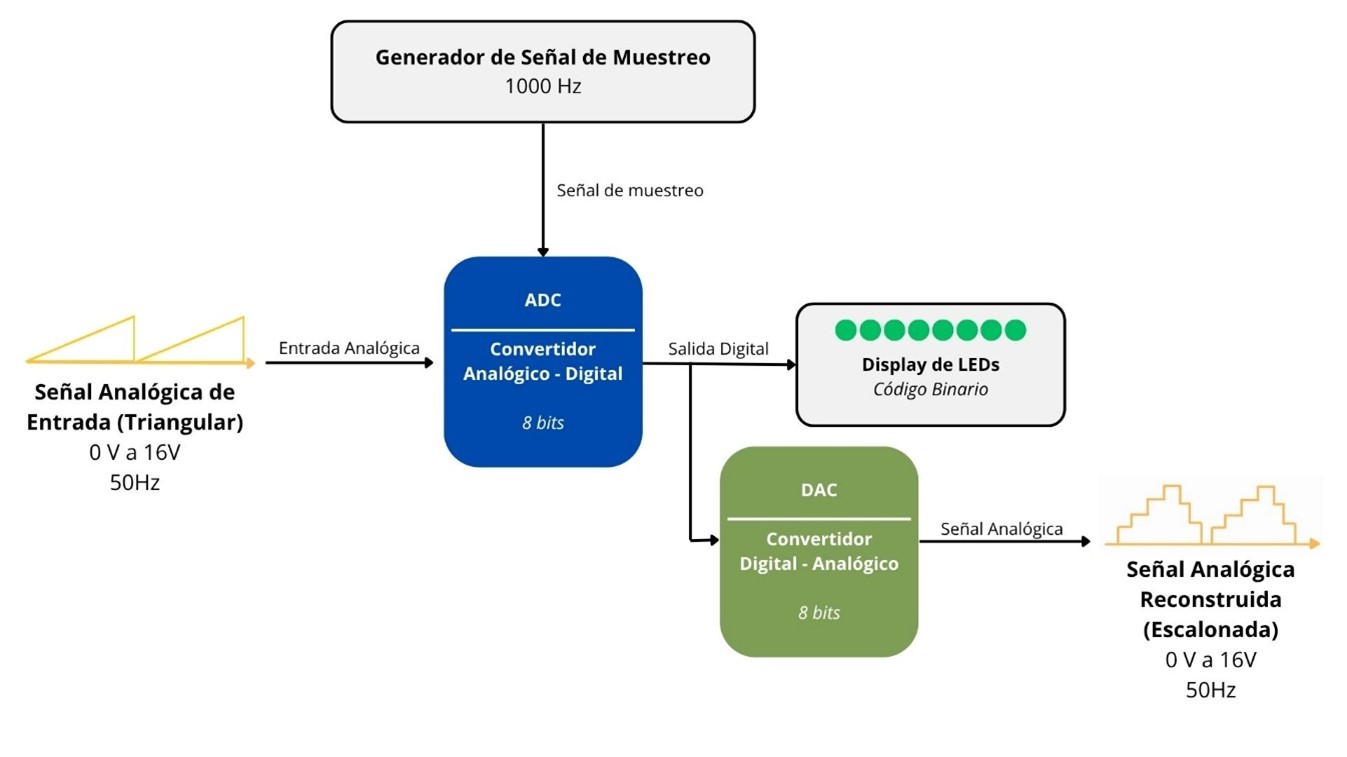
\includegraphics[width=0.7\linewidth]{Img/Esquema.jpg}
        \caption{Esquema general correspondiente a la simulación}
        \label{fig:EsqGeneral}
    \end{figure}

    En la Figura \ref{fig:EsqGeneral} se observa que la señal triangular de entrada es aplicada al convertidor ADC, mientras que la señal de muestreo define los instantes en los cuales se realiza cada conversión. Como resultado, se obtiene una salida digital correspondiente a un valor binario proporcional al voltaje de entrada en cada instante de muestreo. Posteriormente, dicha salida digital es enviada al convertidor DAC, permitiendo reconstruir una señal analógica similar a la original, aunque con forma escalonada.

    \subsection{Resolución del ADC}

    Para analizar el comportamiento del sistema, se calcula la resolución del convertidor, la cual corresponde al cambio mínimo de voltaje que puede ser representado utilizando la ecuacion \ref{Eq:Vres}:
    
    Usando:
    
    \begin{itemize}
        \item $V_{max} = 16 \, V$
        \item $V_{min} = 0 \, V$
        \item $n = 8 \, bits$
    \end{itemize}
    
    Reemplazando:
    
    \[
    V_{res} = \frac{16 - 0}{256} = 0,0625 \, V
    \]
    
    De acuerdo con lo anterior, cada incremento en el valor digital representa aproximadamente 0,0625 V, lo que define la precisión del sistema.

    \subsection{Frecuencia de muestreo}

    De acuerdo con lo solicitado, el sistema tiene un frecuencia $f_{in}$ de 50 Hz y se requiere obtener 20 muestras por ciclo de la señal de entrada. La frecuencia de muestreo $f_s$ se calcula utilizando la siguiente fórmula \ref{Eq:fs}:
    
    Donde utilizando:
    
    \begin{itemize}
        \item $f = 50 \, Hz$
        \item $N = 20 \, muestras$
    \end{itemize}
    
    Reemplazando:
    
    \[
    f_s = 50 \times 20 = 1000 \, Hz
    \]
    
    Además, considerando que la señal de entrada posee una frecuencia de 50 Hz, cada ciclo tiene una duración de 20 ms.
    
    Según este resultado, la frecuencia de muestreo utilizada permite obtener las muestras necesarias para representar correctamente la señal de entrada.

    \subsection*{Relación entre el voltaje de entrada y la salida digital}

    La relación entre el voltaje de entrada y el valor digital generado por el ADC se puede expresar mediante la ecuación \ref{Eq:D10}:
    
    Donde utilizando:
    
    \begin{itemize}
        \item $V_{in} = \text{Voltaje de entrada}$
        \item $V_{min} = 0 \, V$
        \item $V_{res} = 0,0625 \, V$
    \end{itemize}

    Reemplazando:

    \[
        D_{10} = \frac{V_{in}}{0,0625}
    \]

    Esta ecuación permite determinar el código decimal asociado a cada valor de entrada dentro del rango de operación del ADC.

    \subsection{Resultados esperados}

    A partir del análisis teórico, se espera que el convertidor ADC entregue un código binario proporcional al voltaje instantáneo de la señal triangular de entrada. En particular:
    
    \begin{itemize}
        \item Para $V_{in} \approx 0 \, V \rightarrow$ código mínimo \textbf{00000000}
        \item Para valores intermedios $\rightarrow$ aumento progresivo del código binario
        \item Para $V_{in} \approx 16 \, V \rightarrow$ código máximo \textbf{11111111}
    \end{itemize}
    
    Además, se espera que la señal digital resultante presente una forma escalonada, producto del proceso de cuantización propio del ADC.
    
    Por otra parte, al conectar la salida digital al convertidor DAC, se espera obtener una señal analógica similar a la señal triangular original, aunque con forma escalonada debido al proceso de reconstrucción por niveles discretos.
    
    Como ejemplo, para un voltaje de entrada $V_{in} = 10V$ y utilizando la ecuación anteriormente planteada:
    
    \[
    D_{10} = \frac{10}{0,0625} = 160
    \]
    
    El valor decimal 160 corresponde al código binario:
    
    \begin{center}
        \textbf{10100000}
    \end{center}
    
    Este resultado es coherente con el comportamiento esperado del ADC y permite su comparación con los valores obtenidos en la simulación, verificando así el correcto funcionamiento del sistema diseñado.

    Para el DAC, se espera que la señal reconstruida siga el comportamiento general de la señal original, aunque con una forma escalonada propia del proceso de conversión digital-analógica. Utilizando la ecuación \ref{Eq:Vout}, se puede calcular el voltaje de salida correspondiente al \enquote{escalón} generado por el DAC para el código binario $1010 0000_2 = 160_{10}$:

    Donde utilizando:
    \begin{itemize}
        \item $V_{ref} = 16 \, V$
        \item $D = 160$
        \item $n = 8$
    \end{itemize}

    Reemplazando:
    \[
        V_{out} = 160 \times \frac{16}{256} \rightarrow 160 \times 0.0625 =  10.0 \, V
    \]

    \subsection{Análisis del diseño}

    El sistema diseñado permite convertir una señal analógica en una señal digital y posteriormente reconstruirla nuevamente como señal analógica, cumpliendo con el funcionamiento esperado de un sistema ADC/DAC.
    
    La resolución del ADC define qué tan preciso es el sistema, ya que indica el cambio mínimo de voltaje que se puede representar. Debido a esto, existe un pequeño error llamado cuantización, ya que no todos los valores analógicos pueden representarse exactamente.
    
    Por otra parte, la frecuencia de muestreo utilizada (1000 Hz) permite tomar suficientes muestras de la señal en cada ciclo, lo que asegura que la forma triangular de entrada se represente de buena manera.
    
    Además, se observa que la salida digital aumenta a medida que aumenta el voltaje de entrada, lo que demuestra que el sistema funciona de forma coherente.
    
    Respecto al DAC, se espera que la señal reconstruida siga el comportamiento general de la señal original, aunque con una forma escalonada propia del proceso de conversión digital-analógica.
    
    En conjunto, este análisis permite tener una base para comparar con los resultados de la simulación y comprobar que el sistema funciona correctamente.



    \newpage

    \section{Simulación del circuito}

    A continuación, se presenta la simulación del circuito diseñado anteriormente, la cual fue realizada utilizando el software Multisim (14.1). El objetivo de esta etapa es verificar el correcto funcionamiento del sistema y comparar los resultados obtenidos con el análisis teórico. El Circuito implementado se muestra en la Figura \ref{fig:Simulacion}, donde se pueden identificar claramente los bloques funcionales descritos en la sección anterior.

    Antes de adentrarse en la simulación es fundamental definir los puertos que conforman tanto al ADC como al DAC.

    \textbf{-ADC}:
    \begin{itemize}
        \item $V_{in}$: Entrada analógica (señal triangular diente sierra)
        \item $V_{ref+}$: Voltaje de referencia positivo (16 V)
        \item $V_{ref-}$: Voltaje de referencia negativo (0 V)
        \item SOC: Señal de muestreo (1000 Hz)
        \item $D_0$ a $D_7$: Salidas digitales (código binario de 8 bits)
    \end{itemize}
        
    \textbf{-DAC}:
    \begin{itemize}
        \item $D_0$ a $D_7$: Entradas digitales (código binario de 8 bits)
        \item $V_{out}$: Salida analógica reconstruida
        \item $V_{ref+}$: Voltaje de referencia positivo (16 V)
        \item $V_{ref-}$: Voltaje de referencia negativo (0 V)
    \end{itemize}

    \begin{figure}[H]
        \centering
        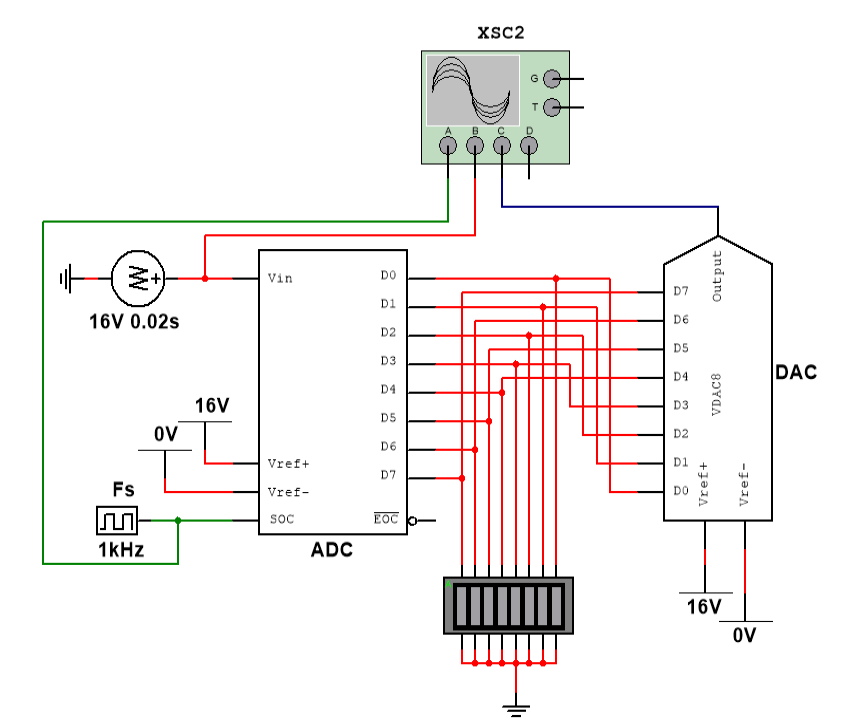
\includegraphics[width=0.6\linewidth]{Img/SimGen.png}
        \caption{Simulación del circuito ADC/DAC en Multisim}
        \label{fig:Simulacion}
    \end{figure}

    Dentro del simulador, se comprobó que el sistema realiza 20 muestras por ciclo de la señal triangular y los 20 \enquote{escalones} correspondiente al DAC, tal como se había establecido en el diseño teórico. Para ello, se simulo un periodo completo de la señal de entrada y se observaron los pulsos en el osciloscopio.
    
    \begin{figure}[H]
        \centering
        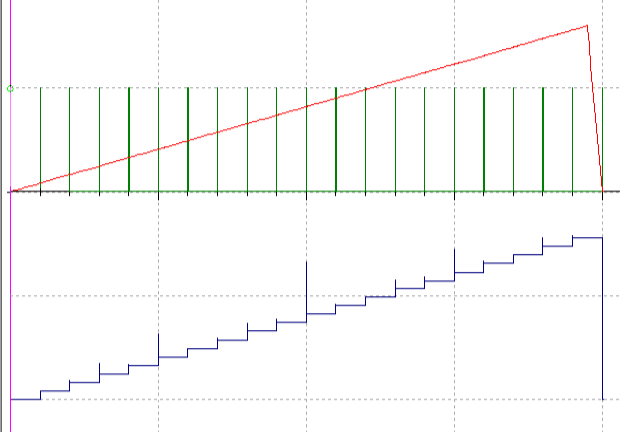
\includegraphics[width=0.6\linewidth]{Img/Muest.png}
        \caption{Visualización de la señal de entrada, pulsos de muestreo y señal reconstruida en el osciloscopio}
        \label{fig:Osciloscopio}
    \end{figure}

    En la Figura \ref{fig:Osciloscopio} se puede observar la señal triangular de entrada (en rojo) y los pulsos de muestreo (en verde) que indican los momentos en que el ADC toma las muestras. Se verifica que se cumplen las 20 muestras por ciclo, lo que coincide con lo establecido en el diseño del sistema, ademas de asegurar una configuración adecuada en el sistema de muestreo.

    Una vez comprobado que el sistema realiza correctamente las 20 muestras por ciclo (ADC), se procedió a analizar la señal digital resultante en los LEDs y la señal analógica reconstruida por el DAC, comparándolas con la señal de entrada original.

    Para esto, se analizaron distintos puntos de la señal de entrada y verificando que el código binario entregado por el ADC corresponda con el valor esperado según las ecuaciones planteadas en el análisis teórico. Ademas, se verifico que la señal escalonada que entrega el DAC concuerda con el ADC.

    \subsection{\textbf{\textit{Caso 1: Máximo}}}

    En este caso, se analizó el pulso máximo que recibe el ADC, para esto, se configuro para que la simulación se detenga a los 19,5 ms (antes de terminar el primer ciclo). El resultado se muestra en la Figura \ref{fig:Max}.

    \begin{figure}[H]
        \centering
        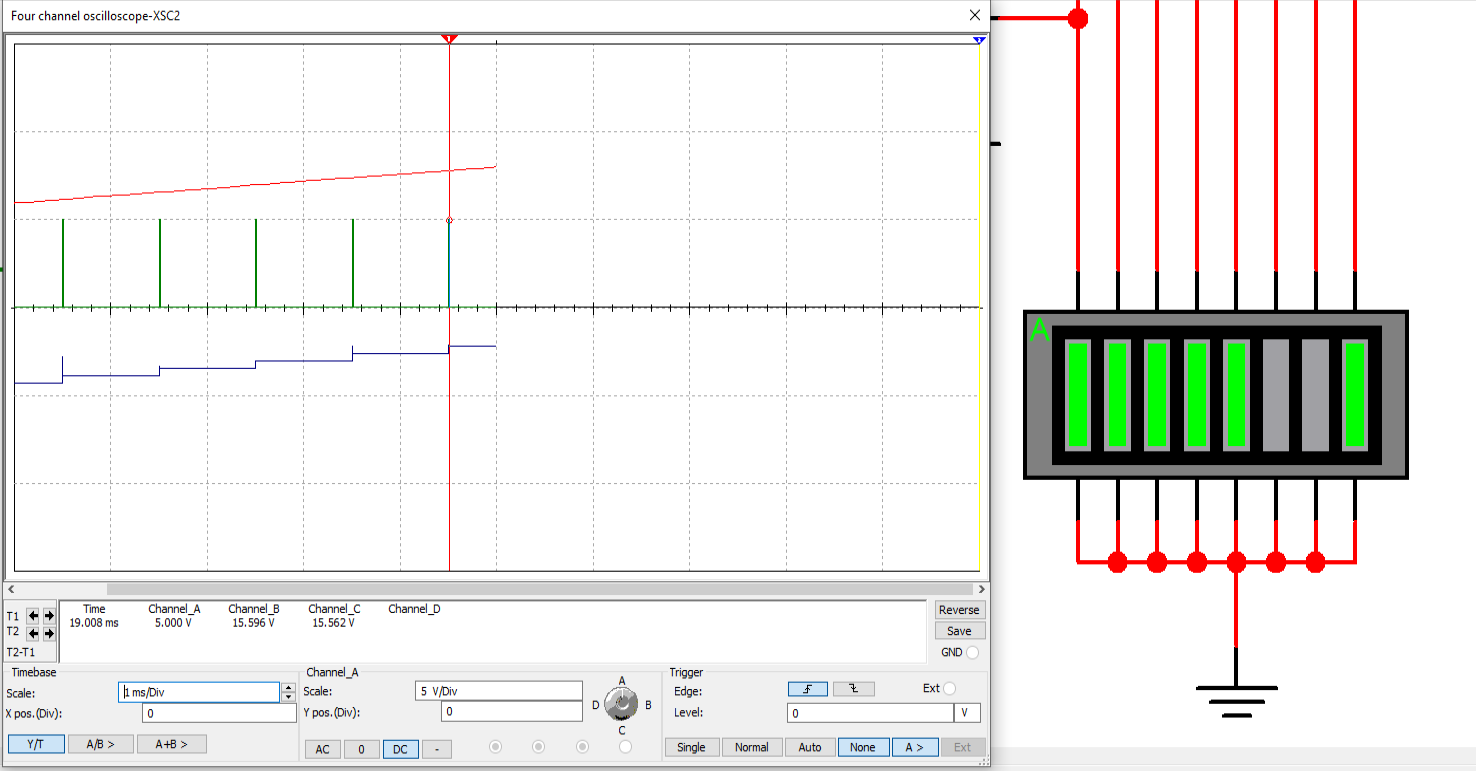
\includegraphics[width=0.8\linewidth]{Img/Max.png}
        \caption{Análisis del caso máximo}
        \label{fig:Max}
    \end{figure}

    Como se observa en el osciloscopio, el voltaje obtenido se encuentra dado por en T1/Chanel\_B, el cual corresponde a un valor de \textbf{15.596V} ($V_{in}$). Para verificar que el código binario entregado por el ADC corresponde a este valor, se realizan las siguientes operaciones:

    Según los datos obtenidos previamente:

    \begin{itemize}
        \item $V_{in} = 15.596 \, V$
        \item $V_{min} = 0 \, V$
        \item $V_{res} = 0.0625 \, V$
    \end{itemize}

    $$D_{10} = \frac{15.596 - 0}{0.0625} \approx 249.536$$

    $$249_{10} = 1111 1001_2$$

    Este resultado coincide exactamente con la barra de LEDs, donde se observan los bits correspondientes en estado lógico alto (encendidos), validando así el correcto funcionamiento del ADC en este punto de la señal de entrada. 

    Para verificar la señal reconstruida por el DAC utilizando el código binario obtenido, se realiza el proceso inverso:

    \begin{itemize}
        \item $D_{10} = 249$
        \item $V_{res} = 0.0625 \, V$
    \end{itemize}

    $$V_{out} = D_{10} \times \frac{V_{ref}}{256} = 249 \times 0.0625 = 15.5625 V$$

    Al contrastar este cálculo con la simulación, se observa que la señal de color azul mostrada en el osciloscopio (T1/Chanel\_C) corresponde a un valor de \textbf{15.562 V}, lo cual es consistente con el valor calculado anteriormente, confirmando que el DAC está reconstruyendo la señal de manera adecuada. 





    \newpage

    \subsection{\textbf{\textit{Caso 2: Mínimo}}}

    En este caso, se analizó el pulso mínimo que recibe el ADC, para esto, se configuro para que la simulación se detenga a los 20,5 ms (justo después de terminar el primer ciclo). El resultado se muestra en la Figura \ref{fig:Min}.

    \begin{figure}[H]
        \centering
        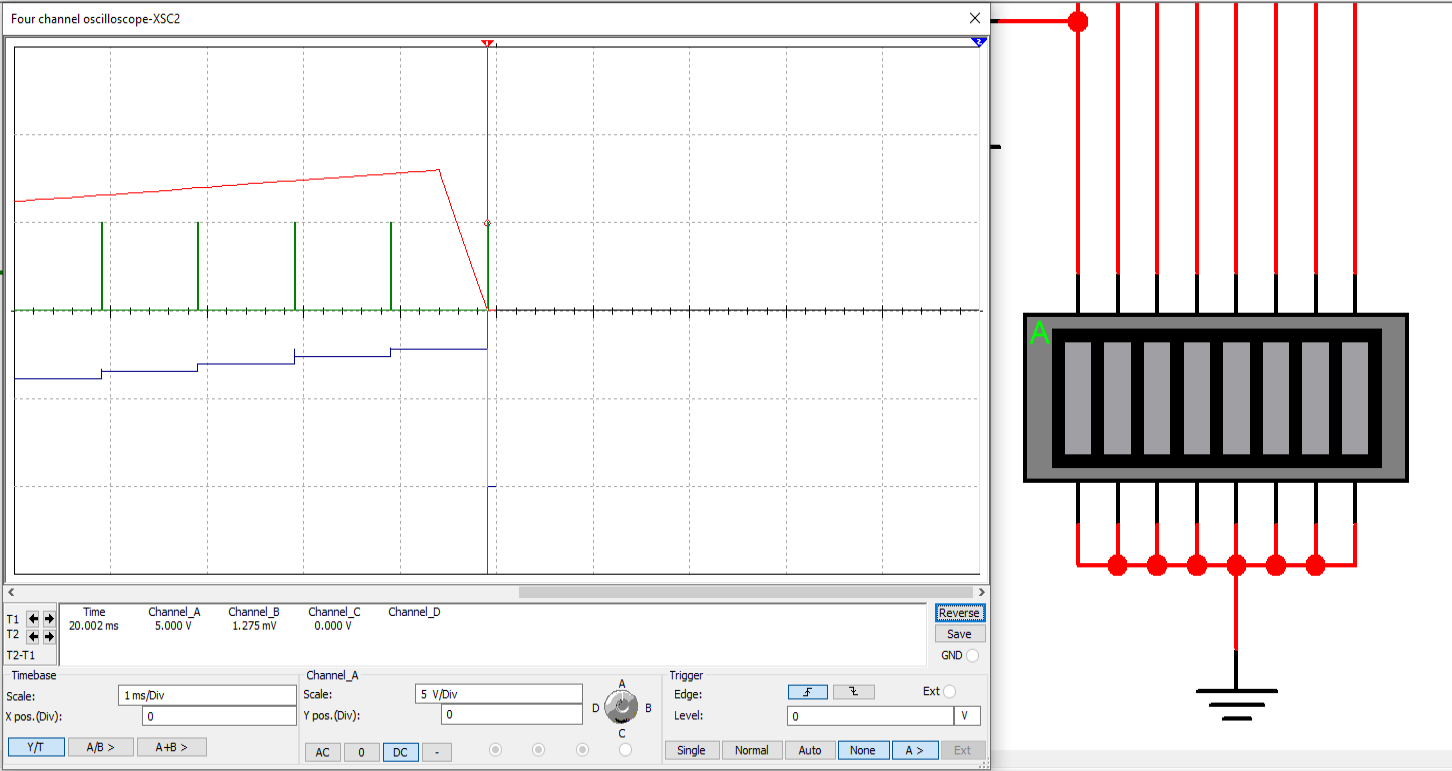
\includegraphics[width=0.6\linewidth]{Img/Min.png}
        \caption{Análisis del caso mínimo}
        \label{fig:Min}
    \end{figure}

    Como se observa en el osciloscopio, el voltaje obtenido se encuentra dado por en T1/Chanel\_B, el cual corresponde a un valor de \textbf{0.004V} ($V_{in}$). Para verificar que el código binario entregado por el ADC corresponde a este valor, se realizan las siguientes operaciones:

    \begin{itemize}
        \item $V_{in} = 1.275 \, mV \Rightarrow  0.001275 \, V$
        \item $V_{min} = 0 \, V$
        \item $V_{res} = 0.0625 \, V$
    \end{itemize}

    $$D_{10} = \frac{V_{in} - V_{min}}{V_{res}} = \frac{0 - 0}{0.0625} = 0$$

    $$0_{10} = 0000 0000_2$$
    
    Este resultado coincide exactamente con la barra de LEDs, donde se observan todos los bits apagados, validando así el correcto funcionamiento del ADC en este punto de la señal de entrada.

    Para verificar la señal reconstruida por el DAC utilizando el código binario obtenido, se realiza el proceso inverso:

    \begin{itemize}
        \item $D_{10} = 0$
        \item $V_{res} = 0.0625 \, V$
    \end{itemize}

    $$V_{out} = D_{10} \times \frac{V_{ref}}{256} = 0 \times 0.0625 = 0 V$$

    Al contrastar este cálculo con la simulación, se observa que la señal de color azul mostrada en el osciloscopio (T1/Chanel\_C) corresponde a un valor de \textbf{0 V}, lo cual es consistente con el valor calculado anteriormente, confirmando que el DAC está reconstruyendo la señal de manera adecuada.

    \subsection{\textbf{\textit{Caso 3: Punto arbitrario}}}

    En este caso, se analizó un punto arbitrario de la señal de entrada, para esto, se pauso la simulación en un instante arbitrario dentro del primer ciclo. El resultado se muestra en la Figura \ref{fig:Arb}.

    \begin{figure}[H]
        \centering
        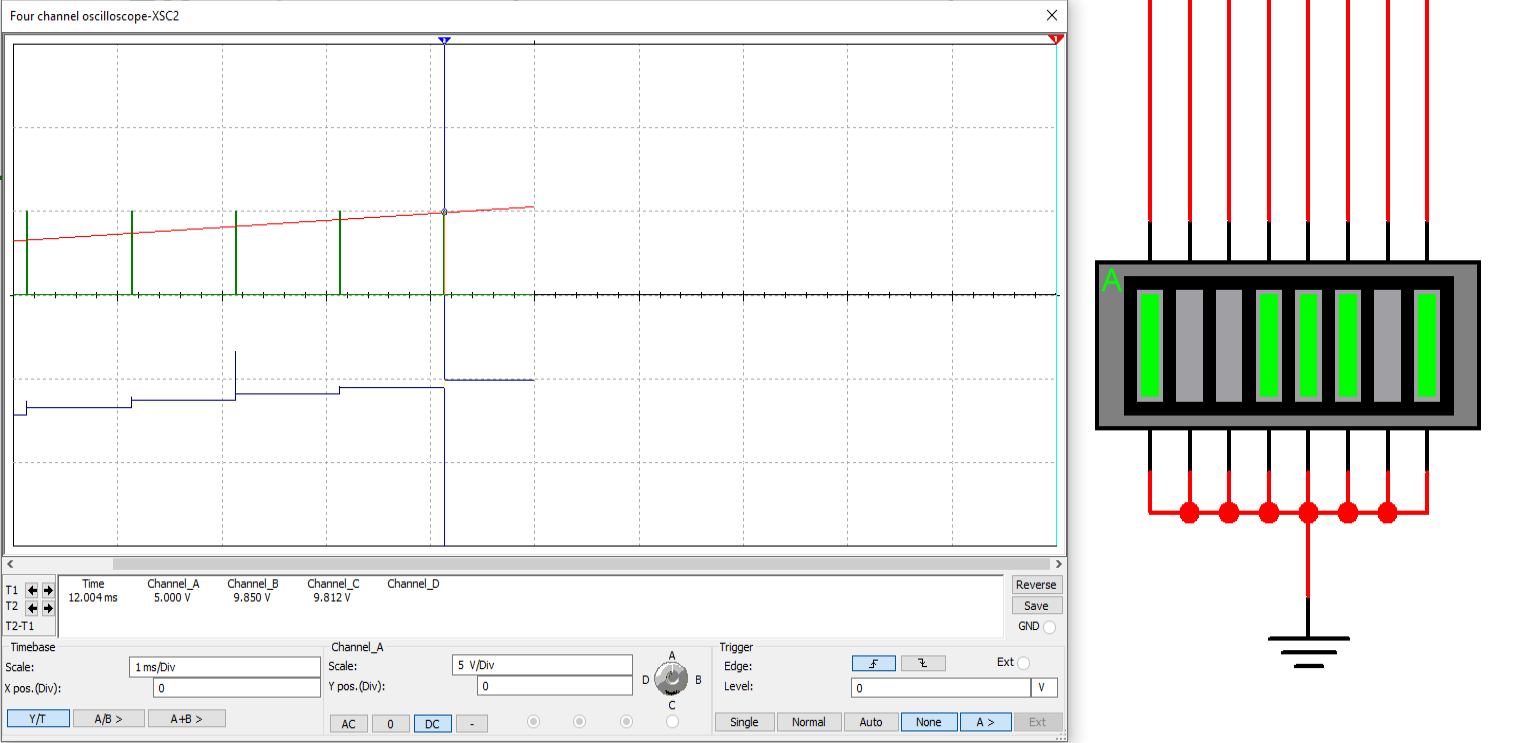
\includegraphics[width=0.6\linewidth]{Img/Arb.png}
        \caption{Análisis de un punto arbitrario}
        \label{fig:Arb}
    \end{figure}

    Como se observa en el osciloscopio, el voltaje obtenido se encuentra dado por en T1/Chanel\_B, el cual corresponde a un valor de \textbf{9.850V} ($V_{in}$). Para verificar que el código binario entregado por el ADC corresponde a este valor, se realizan las siguientes operaciones:

    \begin{itemize}
        \item $V_{in} = 9.850 \, V$
        \item $V_{min} = 0 \, V$
        \item $V_{res} = 0.0625 \, V$
    \end{itemize}

    $$D_{10} = \frac{V_{in}}{V_{res}} = \frac{9.850}{0.0625} = 157.6$$

    $$157_{10} = 1001 1101_2$$

    Este resultado coincide exactamente con la barra de LEDs, donde se observan los bits correspondientes en estado encendidos, validando así el correcto funcionamiento del ADC en este punto de la señal de entrada.

    Para verificar la señal reconstruida por el DAC utilizando el código binario obtenido, se realiza el proceso inverso:
    
    \begin{itemize}
        \item $D_{10} = 157$
        \item $V_{res} = 0.0625 \, V$
    \end{itemize}

    $$V_{out} = D_{10} \times \frac{V_{ref}}{256} = 157 \times 0.0625 = 9.8125 V$$

    Este resultado es consistente con el valor indicado en la simulación, donde la señal de color azul mostrada en el osciloscopio (T1/Chanel\_C) corresponde a un valor de \textbf{9.812 V}, confirmando que el DAC está reconstruyendo la señal de manera adecuada.

    \newpage

    \section{Conclusión}

    El presente laboratorio permitió comprender y validar el funcionamiento de un sistema 
    de conversión analógico-digital y digital-analógico (ADC/DAC), demostrando cómo una 
    señal física continua puede ser digitalizada, procesada y posteriormente reconstruida 
    como señal analógica, cerrando el ciclo completo de conversión presente en los sistemas 
    electrónicos modernos.

    Una observación central fue la diferencia fundamental entre las tres señales involucradas 
    en el proceso. La señal triangular diente sierra original varía de forma continua, pudiendo 
    adoptar infinitos valores dentro de su rango. La señal digital, en cambio, solo representa 
    256 niveles discretos determinados por la resolución de 8 bits del convertidor. Finalmente, 
    la señal reconstruida por el DAC no es una rampa perfectamente lineal sino una escalera 
    de niveles constantes, donde la diferencia entre el valor analógico real y el nivel discreto 
    asignado constituye el error de cuantización, cuya magnitud máxima es de 0,03125 V 
    en este sistema.

    Desde el punto de vista del ADC, el Teorema de Nyquist-Shannon resultó fundamental 
    para garantizar una representación fiel de la señal. Con una frecuencia de muestreo de 
    1000 Hz frente a una señal de 50 Hz, se obtuvieron 20 muestras por ciclo, superando 
    el mínimo teórico requerido. Los tres casos analizados —máximo, mínimo y punto 
    arbitrario— confirmaron que los códigos binarios entregados por el ADC coinciden con 
    los valores calculados teóricamente, con discrepancias dentro del margen esperado del 
    error de cuantización.

    Respecto al DAC, la señal reconstruida siguió el comportamiento general de la señal 
    original en todos los casos verificados, con voltajes de salida consistentes con los 
    valores calculados. Esta comparación entre la señal continua original y la señal 
    escalonada reconstruida ilustra la pérdida de información inherente a la digitalización 
    y refuerza la importancia de comprender estos conceptos para el desarrollo de sistemas 
    informáticos capaces de interactuar con el entorno físico de manera precisa y confiable.


\end{document}
